
\title{%
  Project Proposal\\
  \large High Frequency Trading \\
    Designing Ultra-low-latency Direct Market Access Technologies}


\date{}

\documentclass[12pt]{article}

\usepackage{hyperref}
\hypersetup{
    colorlinks=true,
    linkcolor=blue,
    filecolor=magenta,      
    urlcolor=cyan,
}
\usepackage{graphicx}
\usepackage{enumitem}
\usepackage{hyperref}
\usepackage{listings}

\begin{document}
\maketitle

\begin{abstract}
I chose to focus my last project on the High Frequency Trading (HFT) and Direct Market Access (DMA). I will focus the project's coding on
\href{https://bitcoin.org/en/}{Bitcoin}. However, I will carry out the research into normal (reputable) markets as required in the project. The choice for the Bitcoin is justified in details in the report, however the main reason is that many cryptocurrency exchanges allow for DMA for free via the Internet. Standard financial markets do not this. Nevertheless, modelling the market order book is very similar for every assets. I will focus on working with the order book (level 2) data. I personally do not see into cryptocurrencies much and I do not seek to promote them in any way.
\end{abstract}


\section{Project Aims}
\label{sec:Aims}
This is provided in the WQU notes.
\begin{itemize}
\item Identify the electronic trading chain showing the linkages between
Exchanges, Brokers, Algo. Trading engines, DMA Services, etc.
\item Explicitly identify the benefits and pitfalls of different DMA access
technologies such as Automated Order Routing Systems (AORs),
Sponsored Access (SA), and direct access by non-intermediary market-
members.
\item Classify and suggest ways to handle risks associated with DMA.
\item Classify the different types of latencies (Transmission Latency,
Propagation Latency, Processing Latency, etc.) and suggest ways to
improve on them.
\item Considering a typical Order messaging process (Order Request, Data
Conversion, Order Enrichment, Order Transmission, Exchange
Acknowledgement), suggest the ideal architecture to develop ultra-low
latency systems.
\end{itemize}

\section{Scope of Research Project}
\label{sec:Scope}
This is provided in the WQU notes.
\begin{itemize}
\item Identify specific countries/markets/financial instruments to study. The
instruments chosen should have sufficient liquidity to support high
frequency trading.
\item Collect and collate high frequency data of stock/contract prices for a
representative section of instruments for that market.
\item Devise simple trading strategies/models to successfully demonstrate the
benefits of ultra-low latency trading in the HFT space – all relevant
parameters and metrics of the system should be clearly identified and
backtested.
(Note: Consider realistic trading scenarios.)
\item Analyze performance of such strategies in out of sample data. If relevant
out of sample data is not available, perform a Monte Carlo to simulate the
same.
\item Summarize and draw conclusions.
\end{itemize}

\section{Research - Standard Financial Markets}
This sections details the required research work for the project as in section~\ref{sec:Aims}. My plan is go over the below references and summarise the relevant ideas in my submission. I may add or remove of items of the list however all of the mentioned items seems relevant in some way. I will use the below list to complete the section~\ref{sec:Chian} to~\ref{sec:Messaging}.


\begin{thebibliography}{9}
%  \cite{Template}

%\bibitem{Template}
%Authors
%\textit{Title}.
%publisher, city, year
%
%\bibitem{knuthwebsite} 
%Knuth: Computers and Typesetting,
%\\\texttt{http://www-cs-faculty.stanford.edu/\~{}uno/abcde.html}

\bibitem{Johnson}
Johnson, Barry
\textit{Algorithmic trading \& DMA: An introduction to direct access trading strategies}.
4Myeloma Press, London, UK, 2010

\bibitem{Harris}
Harris, Larry
\textit{Trading and Exchanges: Market Microstructure for Practitioners}.
Oxford University Press, Oxford, 2003

\bibitem{Dacorogna}
Dacorogna, Michel
\textit{An introduction to high-frequency finance}.
Academic Press, San Diego, 2001

\bibitem{narang}
Narang, Rishi
\textit{Inside the black box : the simple truth about quantitative trading}.
Wiley, Hoboken, N.J, 2009

\bibitem{durbin}
Durbin, Michael
\textit{All about high-frequency trading}.
McGraw-Hill, New York, NY, 2010

\bibitem{ice}
Intercontinental Exchange
\\\texttt{https://www.intercontinentalexchange.com/index}

\bibitem{lse}
London Stock Exchange
\\\texttt{https://www.londonstockexchange.com/home/homepage.htm}


\end{thebibliography}


\subsection{Electronic Trading Chain}
\label{sec:Chian}
ToDo, by 18/11/18
\subsubsection{Exchanges}
\subsubsection{Brokers}
\subsubsection{Algo. Trading engines}
\subsubsection{DMA Services}
\subsection{Benefits and Pitfalls of DMA technologies}
ToDo, by 18/11/18
\subsubsection{Automated Order Routing systems - AORs}
\subsubsection{Sponsored Access - SA}
\subsubsection{Direct access by non-intermediary market-members}
\subsection{Risks in DMA}
ToDo, by 18/11/18
\subsection{Latency Types}
ToDo, by 24/11/18
\subsubsection{Transmission Latency}
\subsubsection{Propagation Latency}
\subsubsection{Processing Latency}
\subsection{Typical Order Messaging System}
\label{sec:Messaging}
ToDo, by 24/11/18
\section{Coded Project - Bitcoin}
I will address the requirements for the section~\ref{sec:Scope} - coding.
\subsection{Why Bitcoin?}
The reasons for Bitcoin or cryptocurrencies for this project is that they offer full free DMA over the Internet. I wish to focus on the order market book modelling and creating trading signals from the order market book.
\subsection{Resources}
The cryptocurrency market seems accessible over the Internet mostly. Good start is this exchange comparisons \href{https://coinmarketcap.com/}{website}. We can use it to focus on our attention to exchange such as \href{https://www.binance.com/en}{Binance}. I am not sure how far this exchange or the cryptocurrency market is reputable. We have a risk the exchange would manipulate the trades, however we will not do real trading. For us, it is important to realise that their API is fine for what we need and we have full access to the market book. As a result, cryptocurrency exchanges offer greater transparency with regards to the trading. The normal exchanges never publish their books freely (not even from \href{https://iextrading.com/}{IEX}). The exchange defines Bitcoin \href{https://info.binance.com/en/currencies/bitcoin}{here}.
\subsection{API}
 \href{https://www.binance.com/en}{Binance} offers a public  \href{https://github.com/binance-exchange/binance-official-api-docs/blob/master/rest-api.md}{Rest API}. The Python package for it is 
  \href{https://python-binance.readthedocs.io/en/latest/}{Python-binance}. After a short account setup, we can access the data market order book and trade as well. Using some simple codes proves that I will be able to access the market directly. The example with Bitcoin as quoted in USD (BTCUSDT) is:
\begin{verbatim}
from binance.client import Client
client = Client(API_KEY, API_SECRET)
depth = client.get_order_book(symbol='BTCUSDT')
\end{verbatim}
This gives me a dictionary with keys \textbf{['lastUpdateId', 'bids', 'asks']}. It shows the same information as \href{https://www.binance.com/en/trade/BTC_USDT}{here} as Binance website.

\begin{center}
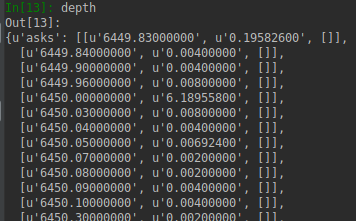
\includegraphics[width=10cm]{book.png}
\end{center}

This means that I will be able to fully and directly access the this specific exchange using some simple Python code or go over the source code for Python-binance package and amend it as needed.

The only drawback is that the API has some time limits. These are important to breach as the exchange push by account suspension for time periods.
 
\subsection{Data Storage}
ToDo, by 18/11/18

I will use either Parquet files or SQLite database file. I will need to decide this.
\subsection{Simple Strategy}
ToDo, by 24/11/18

I will build a strategy based on mean reversion. The mean being the estimated prices as implied by the market order book that represents the balance between the bid and ask placed orders. If this mean price is estimated we can then trade any order that significantly deviate from this estimated. I will have to define what significant means in this context. I will try to cover few ways to compute the price implied by the order book.
\subsection{Strategy Performance}
ToDo, by 24/11/18

I will use standard KPIs as covered by WQU. This maybe required as through the project to establish best strategy.
\subsection{Project Conclusions}
ToDo, to be completed by the end of the project. 

\section{Proposal Summary}
I will focus on this project on DMA and HFT and I will work on real example. I know that the cryptocurrencies are not fully trusted assets however they provide a free DMA.

Some points point that I may not have covered and listed in to rubric are:

\subsection{Importance of the Project}
The importance is to try the real direct market access with real market HFT data for the whole market order book. I will focus on one cryptocurrency pair only. Maybe, I will be able to compare to some traditional market if I will be able to find enough information about the standard markets.

\subsection{Course Knowledge}
The course knowledge I will use is to
\begin{itemize}
\item collect data
\item structure the data locally
\item produce data plots and statistical or market strategy analysis.
\end{itemize}
We have not really covered DMA and as detailed data as I will work with in this project.

\subsection{Expected Issues}
The main challenge will be to handle the data. The HFT data on the full order book are large. In addition, analysing the data is harder than just OHLC data. For example, I do understand the timestamps Binance is using with their trades.


\end{document}